\begin{question}
Using \texttt{pandas} import data stored in \href{https://drive.google.com/file/d/1Uu9lQorvzM-1xwRKPNszaSqlCYAiY-gr/view?usp=sharing}{\texttt{stock\_market.xlsx}}. With the resulting dataframe determine:
\begin{itemize}
\item remove duplicates and missing data (how many rows are left ?);
\item stocks with positive variation;
\item the first five stocks with the lowest price.
\end{itemize}
\end{question}

\cprotEnv\begin{solution}
First load the excel file into a dataframe and look at data structure.

\begin{ipython}
import pandas as pd

df = pd.read_excel("stock_market.xlsx")
print (len(df))
print (df.head())
\end{ipython}
\begin{ioutput}
51

  Symbol                      Name   Price  Change  Change%  Volume (M)  \
0     GE  General Electric Company    6.07   -0.19  -0.0304     142.732
1    NOK         Nokia Corporation    4.78    0.33   0.0742     117.960
2      F        Ford Motor Company    6.61   -0.13  -0.0193     115.394
3   PINS           Pinterest, Inc.   34.29    9.10   0.3613     111.864
4   AAPL                Apple Inc.  425.04   40.28   0.1047      93.574

   Avg Volume (M)  Market Cap (B)
0         102.268          53.132
1          31.296          27.083
2          87.719          26.288
3          15.550          20.110
4          35.035        1821.000
\end{ioutput}
        
If we are not sure that our data is \emph{clean} we should check for duplicates and NaN and take care of them. The \texttt{duplicated} method returns the status of each row (duplicate or not, True or False). If we would like just to see the duplicated entries we could combine the \texttt{duplicated} method with the selection syntax like this:

\begin{ipython}
df[df.duplicated() == True]

   Symbol         Name  Price  Change  Change%  Volume (M)  Avg Volume (M)  \
40    RUN  Sunrun Inc.  36.69    0.02   0.0005      20.113           3.604

    Market Cap (B)
40           4.489
\end{ipython}
        
So it looks like we have just one duplicate and we can remove it:

\begin{ipython}
print ("Before duplicates removal: {}".format(len(df)))
df = df.drop_duplicates()
print ("After duplicates removal: {}".format(len(df)))
\end{ipython}
\begin{ioutput}
Before duplicates removal: 50
After duplicates removal: 50
\end{ioutput}

Then we need to take care of the NaN, again if we want to check the rows with NaN we can select (here the syntax is a little bit more complicated since we need to use \texttt{any} to look for Nan in every column):

\begin{ipython}
df[df.isna().any(axis=1)]
\end{ipython}
\begin{ioutput}
   Symbol                                 Name  Price  Change  Change%  \
23   NCLH  Norwegian Cruise Line Holdings Ltd.  13.64   -0.53  -0.0374
47    NBL                   Noble Energy, Inc.    NaN   -0.23  -0.0225

    Volume (M)  Avg Volume (M)  Market Cap (B)
23      28.402          64.895             NaN
47      18.462          13.535           4.795
\end{ioutput}
        
Since we don't want to artificially modify our sample we just drop rows with NaN:

\begin{ipython}
print ("Before NaN removal: {}".format(len(df)))
df = df.dropna()
print ("After NaN removal: {}".format(len(df)))
\end{ipython}
\begin{ioutput}
Before NaN removal: 51
After NaN removal: 49
\end{ioutput}

The second point asks to determine the companies with a daily positive variation. Clearly we have to apply to the dataframe a selection on the "Change" (or "change\%") column requiring positive values.

\begin{ipython}
pos_var = df[df.loc[:, "Change"] > 0]
print (len(pos_var))
pos_var.head() # just printing the first 5 rows
\end{ipython}
\begin{ioutput}
16

  Symbol                         Name   Price  Change  Change%  Volume (M)  \
1    NOK            Nokia Corporation    4.78    0.33   0.0742     117.960
3   PINS              Pinterest, Inc.   34.29    9.10   0.3613     111.864
4   AAPL                   Apple Inc.  425.04   40.28   0.1047      93.574
6    BAC  Bank of America Corporation   24.88    0.04   0.0016      62.039
8     FB               Facebook, Inc.  253.67   19.17   0.0817      53.030

   Avg Volume (M)  Market Cap (B)
1          31.296          27.083
3          15.550          20.110
4          35.035        1821.000
6          72.793         215.562
8          24.521         723.726
\end{ioutput}
        
So in origin we had 48 stocks and just 16 have a positive variation of its price.

The last question requires to print the first 5 stocks with the lowest prices. In this case it is enough to sort by price the dataframe (ascending) and then just select the first 5 entries.

\begin{ipython}
highest_price = df.sort_values(by=['Price'], ascending=True)[:5]
highest_price
\end{ipython}
\begin{ioutput}
   Symbol                      Name  Price  Change  Change%  Volume (M)  \
25   ABEV               Ambev S. A.   2.68   -0.16  -0.0563      26.136
32    BBD      Banco Bradesco S. A.   4.22   -0.32  -0.0705      22.129
1     NOK         Nokia Corporation   4.78    0.33   0.0742     117.960
15    OPK         OPKO Health, Inc.   5.15   -0.76  -0.1286      35.762
33    MRO  Marathon Oil Corporation   5.49   -0.02  -0.0036      21.249

    Avg Volume (M)  Market Cap (B)
25          36.654          41.999
32          22.046          36.739
1           31.296          27.083
15          17.792           3.450
33          34.098           4.339
\end{ioutput}
\end{solution}

\cprotEnv\begin{question}
Given the following discount factors plot the resulting discount curve, possibly adding axis labels and legend.

\begin{ipython}
dfs = [1.0000, 1.0014, 1.0031, 1.0048,
       1.0066, 1.0145, 1.0227,
       1.0304, 1.0369, 1.0423,
       1.0462, 1.0489, 1.0506, 
       1.0513, 1.0514, 1.0508,
       1.0499, 1.0486, 1.0471,
       1.0455, 1.0437, 1.0418,
       1.0399, 1.0379, 1.0358,
       1.0338, 1.0318, 1.0297,
       1.0277, 1.0256, 1.0235,
       1.0215, 1.0194, 1.0174]

pillars = [datetime.date(2020, 8, 3), datetime.date(2020, 11, 3),
           datetime.date(2021, 2, 3), datetime.date(2021, 5, 3),
           datetime.date(2021, 8, 3), datetime.date(2022, 8, 3),
           datetime.date(2023, 8, 3), datetime.date(2024, 8, 3),
           datetime.date(2025, 8, 3), datetime.date(2026, 8, 3),
           datetime.date(2027, 8, 3), datetime.date(2028, 8, 3),
           datetime.date(2029, 8, 3), datetime.date(2030, 8, 3),
           datetime.date(2031, 8, 3), datetime.date(2032, 8, 3),
           datetime.date(2033, 8, 3), datetime.date(2034, 8, 3),
           datetime.date(2035, 8, 3), datetime.date(2036, 8, 3),
           datetime.date(2037, 8, 3), datetime.date(2038, 8, 3),
           datetime.date(2039, 8, 3), datetime.date(2040, 8, 3),
           datetime.date(2041, 8, 3), datetime.date(2042, 8, 3),
           datetime.date(2043, 8, 3), datetime.date(2044, 8, 3),
           datetime.date(2045, 8, 3), datetime.date(2046, 8, 3),
           datetime.date(2047, 8, 3), datetime.date(2048, 8, 3),
           datetime.date(2049, 8, 3), datetime.date(2050, 8, 3)]
\end{ipython}
\end{question}

\cprotEnv\begin{solution}
\begin{ipython}
import datetime
from matplotlib import pyplot as plt
import matplotlib.dates as mdates

dfs = [1.0, 1.0014, 1.0031, 1.0048, ...]
pillars = [datetime.date(2020, 8, 3), datetime.date(2020, 11, 3), ...]

plt.plot(pillars, dfs, marker="o", label="EUR6M d.f.")

plt.gca().xaxis.set_major_formatter(mdates.DateFormatter('%Y-%m-%d'))
# this one instead rotate labels to avoid superimposition
plt.xticks(rotation=45)
plt.xlabel("Pillar dates")
plt.ylabel("Discount Factors")
plt.grid(True)
plt.legend()
plt.show()
\end{ipython}

\begin{figure}[htb]
\begin{center}
  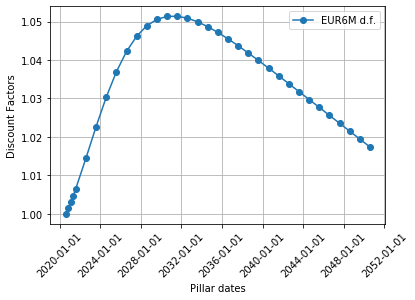
\includegraphics[width=0.7\linewidth]{figures/ex5.5.png}
\end{center}
\end{figure}
\end{solution}



